\documentclass[conference]{IEEEtran}
\IEEEoverridecommandlockouts
\usepackage{cite}
\usepackage{amsmath,amssymb,amsfonts}
\usepackage{algorithmic}
\usepackage{graphicx}
\usepackage{textcomp}
\usepackage{xcolor}
\usepackage{booktabs}
\usepackage{multirow}
\usepackage{url}
\usepackage[hidelinks]{hyperref}

\begin{document}

\title{Cross-Domain Generalization of Personalized Wearable Health\\
State Discovery: A Synthetic-to-Real Evaluation}

\author{
\IEEEauthorblockN{1\textsuperscript{st} Nigam L. Raj}
\IEEEauthorblockA{\textit{Dept. of Information Science and Engineering} \\
\textit{Nitte Meenakshi Institute of Technology}\\
Bengaluru, India \\
nigamraj711@gmail.com}
\and
\IEEEauthorblockN{2\textsuperscript{nd} Prajwal R}
\IEEEauthorblockA{\textit{Dept. of Information Science and Engineering} \\
\textit{Nitte Meenakshi Institute of Technology}\\
Bengaluru, India \\
prajwalgowda81234@gmail.com}
\and
\IEEEauthorblockN{3\textsuperscript{rd} S. Lokesh}
\IEEEauthorblockA{\textit{Dept. of Information Science and Engineering} \\
\textit{Nitte Meenakshi Institute of Technology}\\
Bengaluru, India \\
mail2lokesh022@gmail.com}
\and
\IEEEauthorblockN{4\textsuperscript{th} Sachin S. K}
\IEEEauthorblockA{\textit{Dept. of Information Science and Engineering} \\
\textit{Nitte Meenakshi Institute of Technology}\\
Bengaluru, India \\
sachinsk711@gmail.com}
\and
\IEEEauthorblockN{5\textsuperscript{th} Lakshmi M}
\IEEEauthorblockA{\textit{Dept. of Information Science and Engineering} \\
\textit{Nitte Meenakshi Institute of Technology}\\
Bengaluru, India \\
lakshmi.m@nmit.ac.in}
}

\maketitle

\begin{abstract}
\bfseries Continuous physiological monitoring via consumer wearable devices offers unique opportunities for longitudinal personal health tracking. However, modeling wearable time series is severely complicated by high inter-individual baseline variation, non-stationary daily dynamics, missing data, and an absence of continuous clinical labels. In this paper, we present a leakage-controlled machine learning framework for unsupervised latent health state discovery and dynamic sequence decoding across synthetic and real-world wearable cohorts. By transforming multi-modal signals into personalized 7-day rolling baseline deviations, Gaussian Mixture Models (GMM) discover three macro-level physiological states, followed by Hidden Markov Model (HMM) sequence decoding. Evaluating across 69 real Fitbit users (4,159 daily timelines) and 300 synthetic users (55,200 timelines), zero-shot synthetic-to-real transfer achieves a Silhouette score of 0.2117 $\pm$ 0.0098, closely matching the real-trained baseline (0.2168 $\pm$ 0.0078), with a 2.3\% relative gap that is not statistically significant after Nadeau--Bengio variance correction and Holm--Bonferroni adjustment ($p_{\text{adj}} = 0.1139$). Synthetic data augmentation yields negligible benefit when moderate amounts of real-world training data are available (61 users); all tested augmentation ratios produce small performance decreases relative to real-only training. Non-parametric statistical alignment against Ecological Momentary Assessment (EMA) self-reports ($N = 1{,}751$) reveals an exploratory uncorrected trend in self-reported happiness (\texttt{HAPPY}, $H = 7.0991, p = 0.0287$ uncorrected) that does not survive Holm--Bonferroni correction ($p_{\text{adj}} = 0.2012$).
\end{abstract}

\begin{IEEEkeywords}
Wearable Computing, Unsupervised Learning, Gaussian Mixture Models, Hidden Markov Models, Cross-Domain Transfer.
\end{IEEEkeywords}

\section{Introduction}
Consumer wearable devices such as smartwatches and fitness trackers continuously capture multi-modal physiological streams including resting heart rate, daily physical activity, calorie expenditure, and sleep duration \cite{sano2018, dunn2021}. These longitudinal data streams provide unprecedented granularity for personal health tracking. However, translating raw wearable metrics into actionable physiological insights presents major technical hurdles. First, raw sensor streams exhibit high inter-individual baseline variation; a resting heart rate of 70 BPM may represent elevated physiological stress for an athletic individual but normal baseline for a sedentary user \cite{li2017}. Second, real-world wearable datasets suffer from severe sensor missingness, non-stationary routine shifts, and a complete absence of continuous clinical diagnostic labels \cite{shcherbina2017}.

To address these challenges without relying on supervised clinical targets, unsupervised learning approaches such as Gaussian Mixture Models (GMM) \cite{reynolds2009} and Hidden Markov Models (HMM) \cite{rabiner1989} have emerged as powerful paradigms for latent state discovery \cite{gansbeke2020}. Furthermore, privacy concerns and dataset scarcity make synthetic data generation an attractive alternative for model pre-training. However, whether latent state structures learned from synthetic wearable distributions generalize zero-shot to real-world human physiological timelines remains an open research question.

In this work, we present an end-to-end unsupervised framework for personalized physiological state discovery and cross-domain transfer evaluation. Our core contributions are:
\begin{enumerate}
    \item A causal, leakage-controlled preprocessing framework that converts multi-modal wearable time series into personalized 7-day rolling z-deviations and a harmonized composite severity score.
    \item A comparative four-experiment cross-domain evaluation framework (Synthetic-to-Synthetic, Real-to-Real, Synthetic-to-Real Zero-Shot, and Synthetic+Real Ratio Sweeps), establishing 50-shuffle permutation null baselines for all clustering evaluations.
    \item Rigorous cross-domain statistical evaluation utilizing Nadeau-Bengio \cite{nadeau2003} resampled variance corrections and Holm-Bonferroni \cite{holm1979} multiple-comparison adjustments to benchmark zero-shot transferability and ratio augmentation.
\end{enumerate}

We emphasize that the discovered clusters---interpretively labeled \textit{Recovery}, \textit{Baseline}, and \textit{Strain} by sorting GMM components by median harmonized severity---represent heuristic data-driven proxy labels for exploratory wellness tracking, not clinical diagnoses.

\begin{figure}[t]
\centering
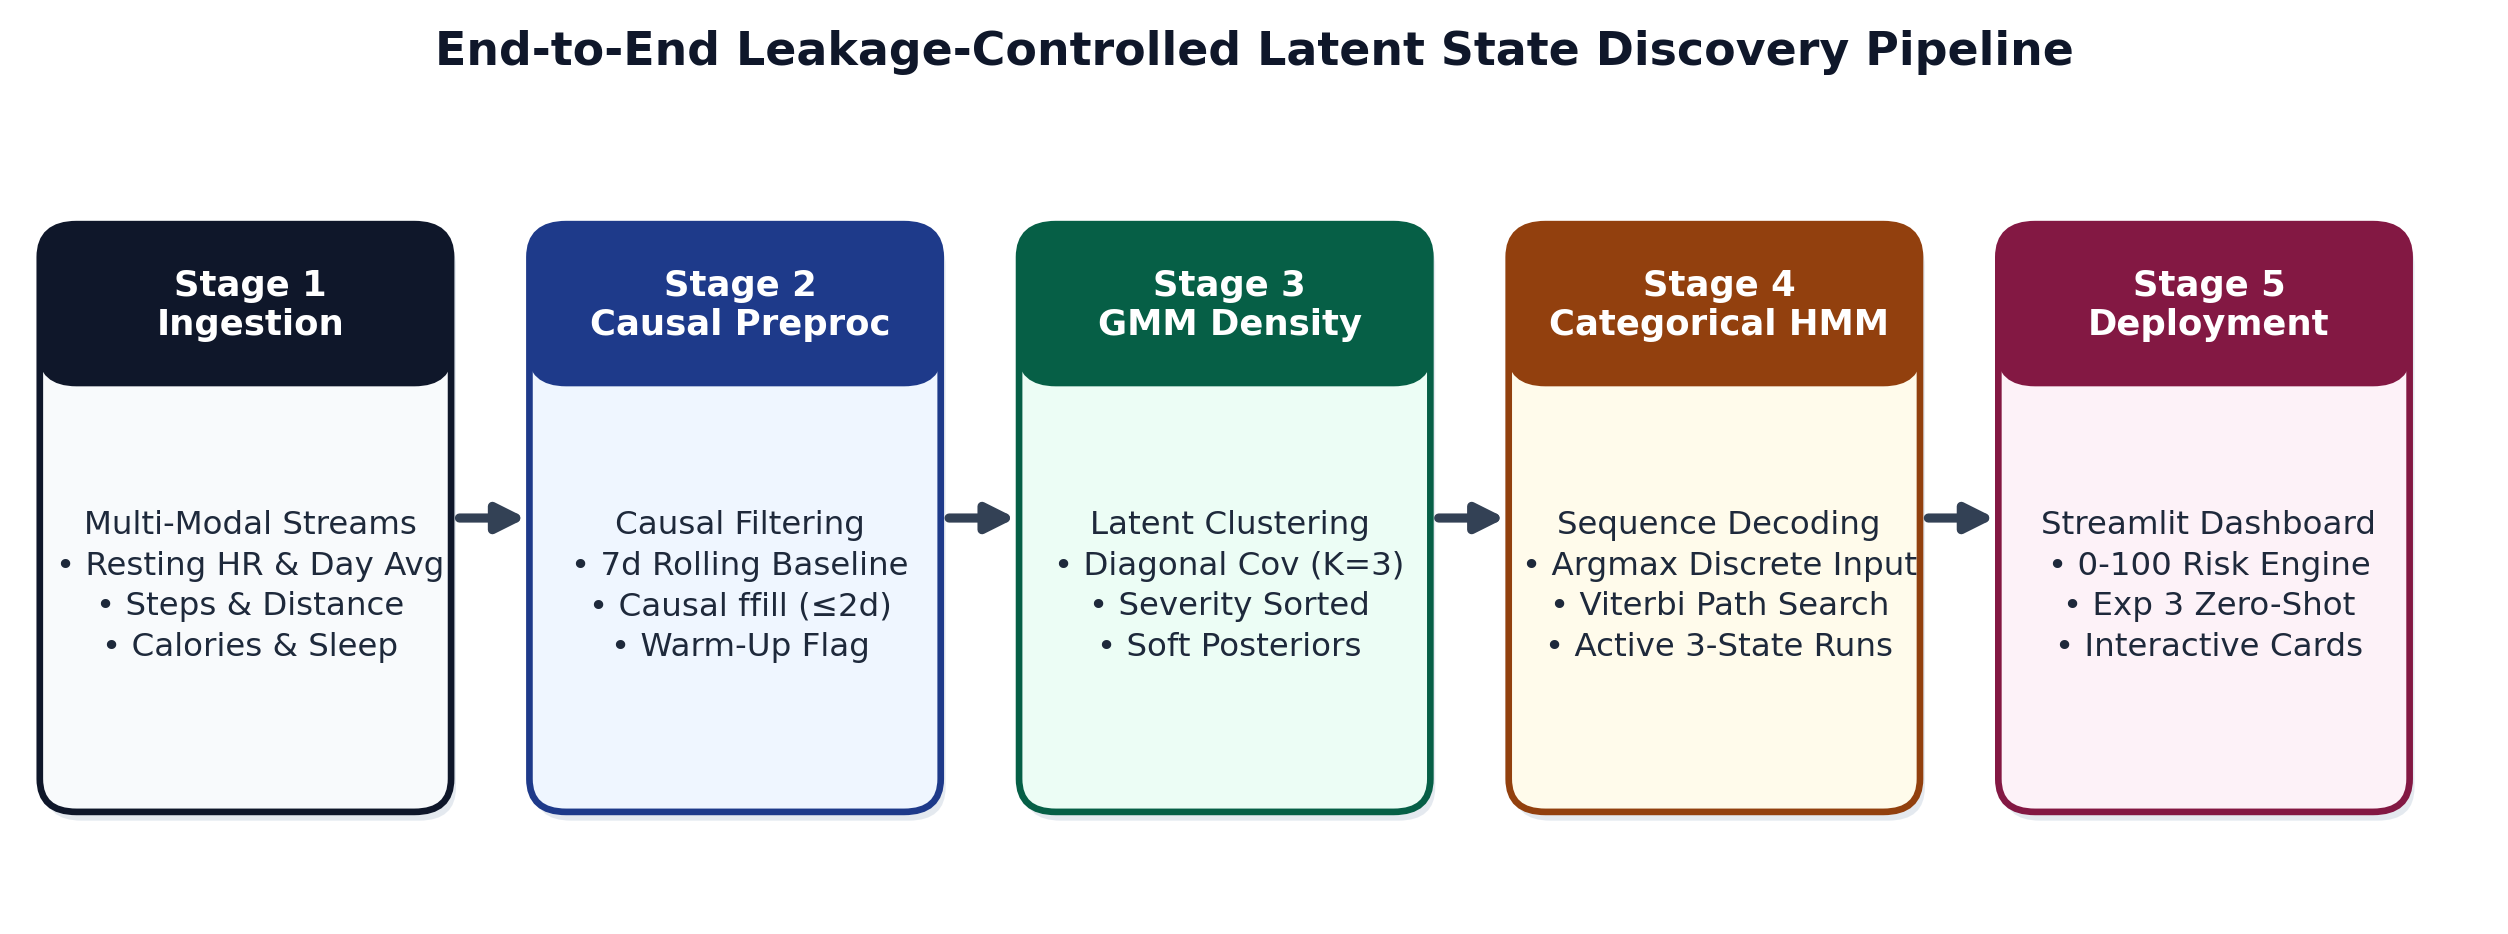
\includegraphics[width=0.48\textwidth]{reports/figures/fig1_pipeline_architecture.png}
\caption{End-to-end leakage-controlled latent state discovery pipeline operating across data ingestion, causal preprocessing, GMM density estimation, HMM sequence decoding, and Streamlit application display.}
\label{fig:pipeline}
\end{figure}

\section{Related Work}
Longitudinal physiological state discovery from wearable sensors builds upon time-series feature engineering and probabilistic sequence modeling \cite{smuck2021}. Prior work has demonstrated that raw physiological metrics fail to generalize across diverse user cohorts due to static demographic offsets \cite{sano2018}. To mitigate baseline heterogeneity, recent studies advocate per-subject z-score normalization over rolling temporal windows \cite{dunn2021}.

Gaussian Mixture Models (GMM) provide a probabilistic framework for soft clustering, estimating continuous posterior probabilities $P(\text{State}_k | x_t)$ that reflect state assignment uncertainty \cite{reynolds2009}. Sequential dynamics are subsequently captured via Hidden Markov Models (HMM), where Viterbi decoding infers optimal latent state sequences over time \cite{rabiner1989}. Clustering quality in unsupervised domain adaptation is typically evaluated using internal validation metrics such as the Silhouette coefficient \cite{rousseeuw1987}, Davies-Bouldin index (DBI) \cite{davies1979}, and Calinski-Harabasz (CH) index \cite{calinski1974}. However, standard statistical comparisons across resampled cross-validation folds often suffer from variance underestimation; Nadeau and Bengio \cite{nadeau2003} formulated a corrected resampled $t$-test to account for non-independence across resamples.

\section{Research Questions and Contributions}
Our experimental evaluation is governed by three locked Research Questions (RQs):
\begin{itemize}
    \item \textbf{RQ1 (In-Domain Baseline Separation)}: Can personalized z-deviation transformations establish statistically meaningful cluster separation ($\text{Silhouette} > \text{Null Floor}$) over raw physiological signals within synthetic and real domains?
    \item \textbf{RQ2 (Zero-Shot Cross-Domain Transfer)}: Does a GMM/HMM pipeline trained exclusively on synthetic control data generalize zero-shot to unseen real-world Fitbit users without catastrophic performance degradation?
    \item \textbf{RQ3 (Synthetic Data Augmentation Sweep)}: Does augmenting real-world training sets with synthetic data at varying ratios ($1:1$, $2:1$, $4:1$) improve downstream clustering separation when real training data is abundant?
\end{itemize}

\section{Dataset and Preprocessing}

\subsection{Synthetic Control Dataset}
The synthetic control dataset comprises 300 longitudinal user timelines totaling 55,200 daily observations (184 days per user). Individual baseline physiological parameters were sampled from population distributions ($\text{RHR}_i \sim \mathcal{N}(64.5, 8.0)$ BPM, $\text{Daytime HR}_i \sim \mathcal{N}(87.1, 10.0)$ BPM, $\text{Steps}_i \sim \mathcal{N}(9282, 2200)$ count, $\text{Distance}_i \sim \mathcal{N}(7.43, 1.8)$ km, $\text{Calories}_i \sim \mathcal{N}(2074, 350)$ kcal, and $\text{Sleep}_i \sim \mathcal{N}(6.99, 1.1)$ hours). Dynamic daily observations incorporate continuous temporal dynamics via a first-order autoregressive process ($\text{AR}(1), \phi=0.65$) with weekend activity shifts ($\pm 12\%$ step/sleep variation) and 5\% uniform random missingness. Crucially, the synthetic generator does \emph{not} hardcode discrete \textit{Recovery/Baseline/Strain} state labels or explicit cluster centroids; latent structure emerges naturally from continuous physiological variance.

\subsection{Real-World Fitbit Cohort and Data Funnel}
The real-world cohort consists of 71 user timelines (7,410 raw records) collected between April 2021 and January 2022. Applying authentic causal filtering yields a primary dataset of 4,159 observations across 69 users (56.13\% row retention, 97.18\% user retention), of which 84.11\% were fully observed and 15.89\% involved conservative causal within-user forward filling of at most two consecutive days. Zero mass cohort-mean imputation was performed. The HMM-eligible sequence subset comprises 4,115 rows across 61 users. Table~\ref{tab:cohort_funnel} presents the unified cohort characteristics and data retention funnel.

\textit{Ethics and Data Availability Disclaimer}: The real dataset's original consent and licensing documentation could not be independently verified from the files available to the authors; the data is used here for non-clinical, academic demonstration purposes only, with no clinical claims made about individual users \cite{birnbaum2020}.

\begin{table}[t]
\caption{Cohort Characteristics and Preprocessing Retention Funnel}
\label{tab:cohort_funnel}
\centering
\begin{tabular}{lrr}
\toprule
\textbf{Cohort & Funnel Property} & \textbf{Synthetic Control} & \textbf{Real Fitbit Cohort} \\
\midrule
Total User Count ($N$) & 300 users & 69 primary (61 HMM) \\
Total Daily Observations & 55,200 rows & 4,159 rows \\
Observation Period & 184 days/user & 283 calendar days \\
Resting HR Mean (BPM) & 64.53 $\pm$ 5.82 & 66.10 $\pm$ 6.24 \\
Daily Steps Mean (count) & 9,282.0 $\pm$ 2,105.4 & 8,448.8 $\pm$ 2,842.1 \\
Sleep Duration Mean (h) & 6.99 $\pm$ 1.12 & 7.43 $\pm$ 1.35 \\
Fully Observed Cells (\%) & 95.00\% & 84.11\% \\
Causal ffill ($\le 2$d) Cells (\%) & 5.00\% & 15.89\% \\
Cohort-Mean Imputed Cells & \textbf{0 (0.00\%)} & \textbf{0 (0.00\%)} \\
\midrule
Raw Export Rows & 55,200 (300u) & 7,410 (71u) [100\%] \\
Primary Complete-Obs & 55,200 (300u) & 4,159 (69u) [56.1\%] \\
HMM Sequence Subset & 55,200 (300u) & 4,115 (61u) [55.5\%] \\
Post-Warmup Analysis Set & 53,100 (300u) & 3,749 (61u) [50.6\%] \\
\bottomrule
\end{tabular}
\end{table}

\subsection{Baseline Models (Severity Terciles and K-Means)}
To test whether latent state discovery captures genuine multivariate structure beyond the composite severity score $S_{i,t} = \frac{1}{6}\sum |z_{i,t,f}|$, we implement a deterministic \textit{Severity-Tercile} baseline. Quantile thresholds ($q_{33}, q_{66}$) are computed exclusively on training-fold user severity distributions ($D_{\text{train}}$) and applied unchanged to held-out test users ($D_{\text{eval}}$). Days with $S_{i,t} \le q_{33}$ are assigned to \textit{Recovery}, $q_{33} < S_{i,t} \le q_{66}$ to \textit{Baseline}, and $S_{i,t} > q_{66}$ to \textit{Strain}. For zero-shot transfer (Exp.~3), synthetic training thresholds are applied directly to real test users with zero real set leakage. For secondary comparison, a hard-assignment $K$-Means ($K=3$) baseline is fit on training-fold scaled deviations ($\mathbf{X}_{\text{train\_scaled}}$) and evaluated on test-fold features ($\mathbf{X}_{\text{eval\_scaled}}$), sorted by median severity score.

\section{Personalized Representation and Severity}

\subsection{Causal Personalized Baseline Extraction}
To prevent look-ahead bias, baseline statistics are calculated causally using a 7-day rolling historical window over preceding observations:
\begin{equation}
\mu_{i,t,f} = \frac{1}{W} \sum_{k=1}^{W} x_{i,t-k,f}, \quad \sigma_{i,t,f} = \sqrt{\frac{1}{W} \sum_{k=1}^{W} (x_{i,t-k,f} - \mu_{i,t,f})^2}
\end{equation}
where $W=7$ days ($\text{min\_periods}=7$). Days 1--6 are explicitly treated as uncalibrated warm-up days. Each raw signal $x_{i,t,f}$ is transformed into a relative z-deviation:
\begin{equation}
Z_{i,t,f} = \frac{x_{i,t,f} - \mu_{i,t,f}}{\sigma_{i,t,f} + \epsilon}
\end{equation}
Figure~\ref{fig:baseline} illustrates the causal baseline extraction and z-deviation transformation process.

\begin{figure}[t]
\centering
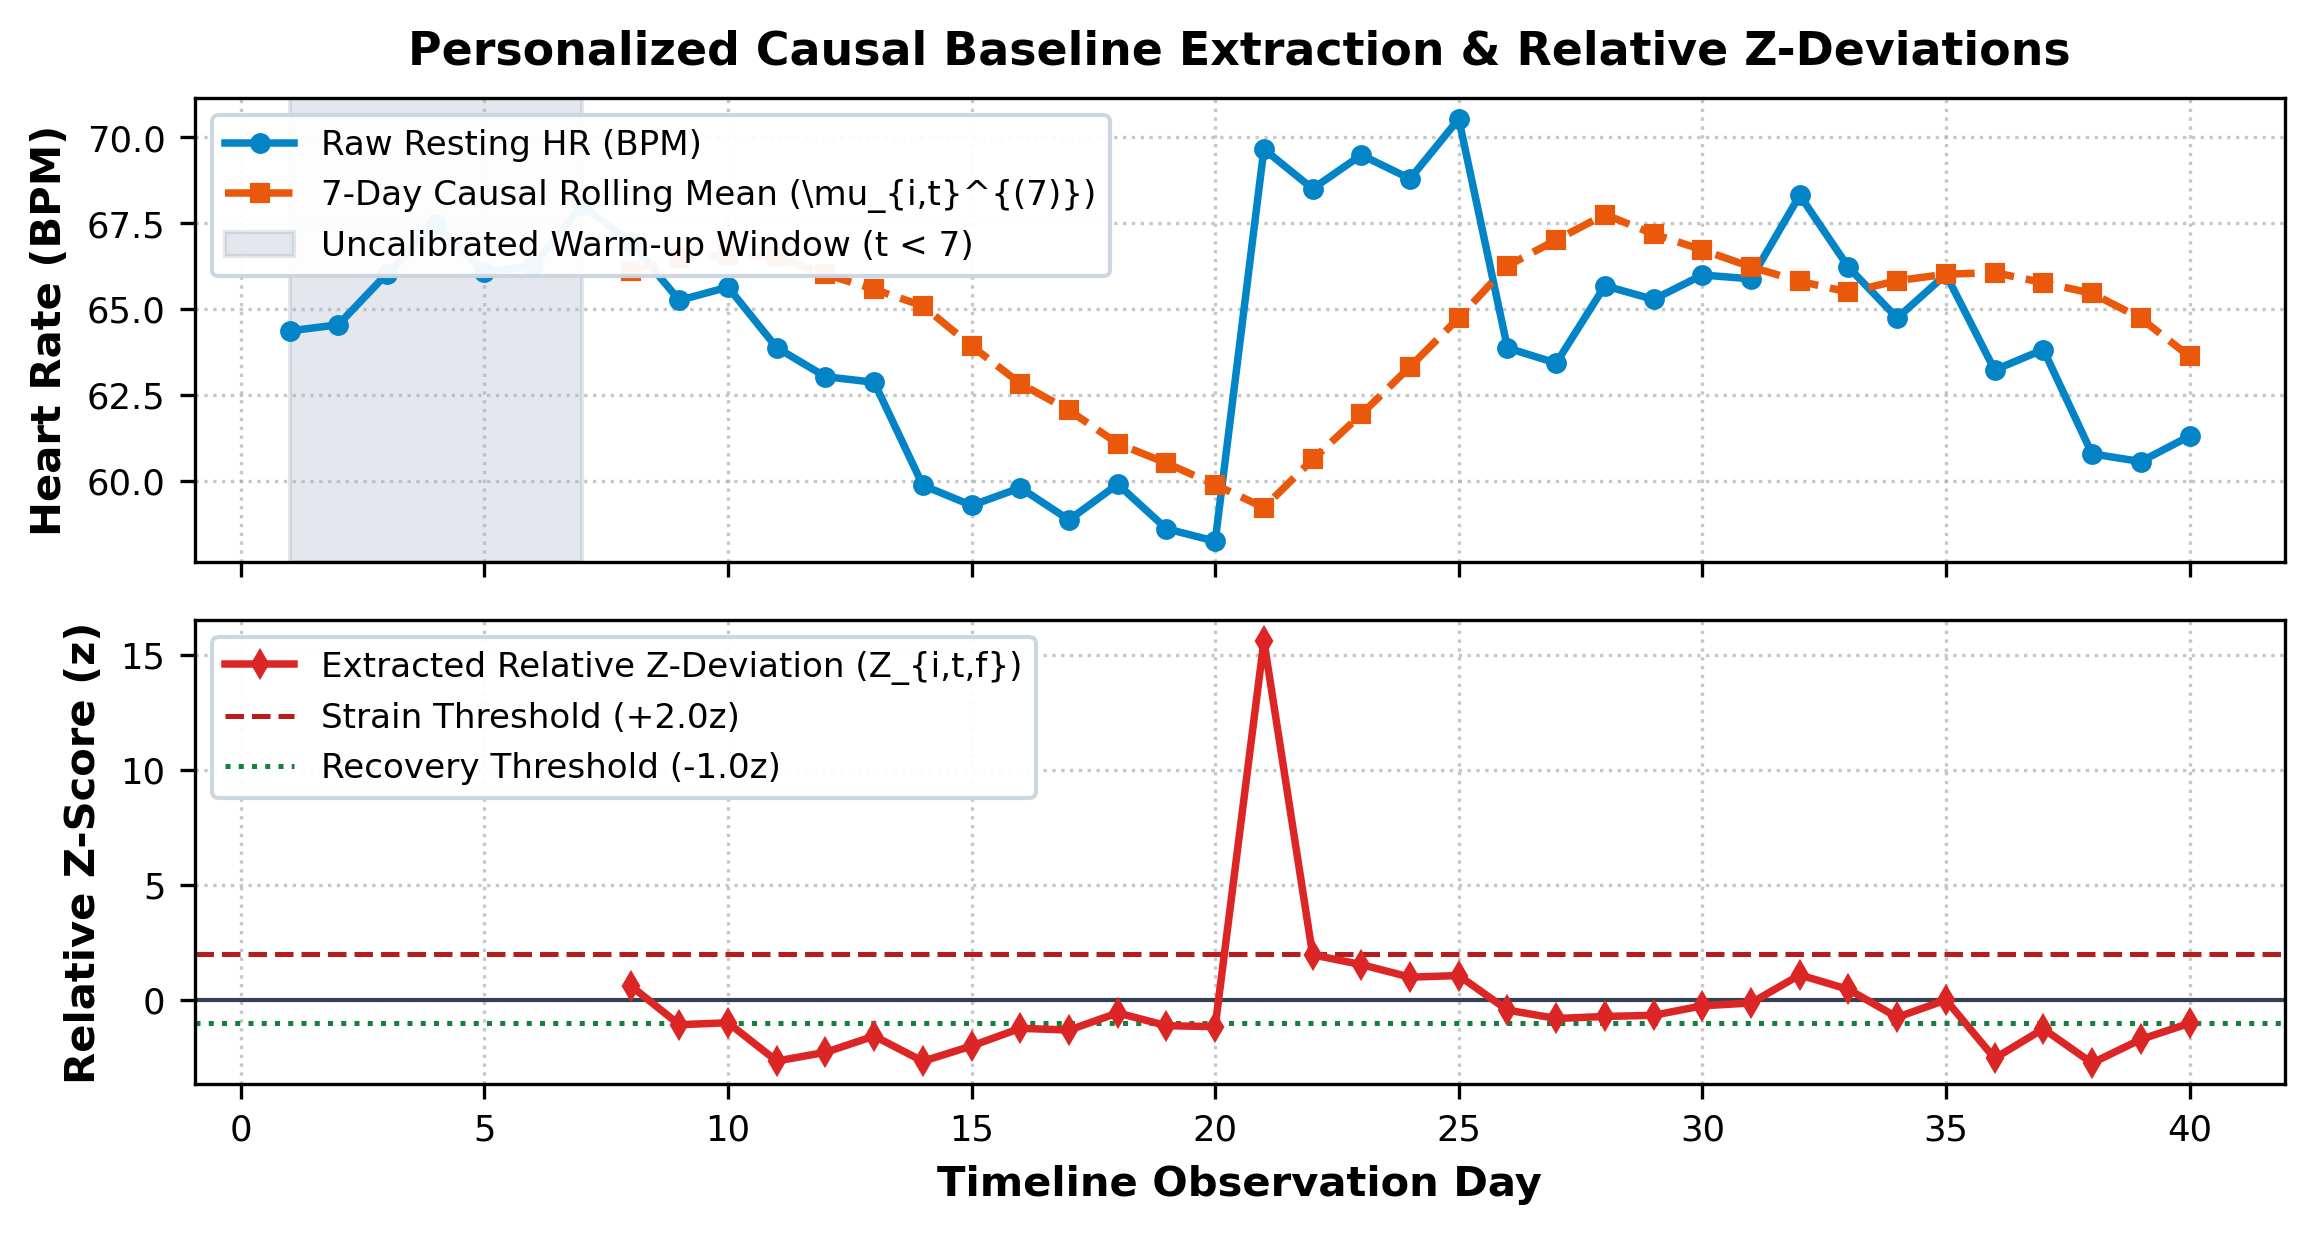
\includegraphics[width=0.48\textwidth]{reports/figures/fig2_personalized_baseline.png}
\caption{Personalized causal baseline calculation showing raw resting heart rate, 7-day causal rolling mean, and extracted relative z-deviation ($z_{i,t}$).}
\label{fig:baseline}
\end{figure}

\subsection{Primary Six-Feature Cross-Domain Harmonization}
The primary cross-domain feature vector contains exactly six harmonized signals common to synthetic and real domains: (1) Resting Heart Rate (\texttt{resting\_hr}), (2) Daytime Average Heart Rate (\texttt{bpm}), (3) Daily Step Count (\texttt{steps}), (4) Walking Distance (\texttt{distance} $/1000$ km), (5) Calorie Expenditure (\texttt{calories} kcal), and (6) Sleep Duration (\texttt{sleep} $/3.6\times 10^6$ hours). The composite homeostatic disruption severity score is mathematically identical across domains:
\begin{equation}
\text{severity\_score}_{i,t} = \sum_{f=1}^{6} |Z_{i,t,f}|
\end{equation}

\section{Latent State Discovery and HMM}

\subsection{GMM Probabilistic Latent State Discovery}
The system uses Gaussian Mixture Models (GMM) with $K=3$ components over scaled z-deviation feature matrices ($\mathbf{f} \in \mathbb{R}^6$). Model-selection sweeps using the Bayesian Information Criterion (BIC) and Akaike Information Criterion (AIC) across candidate cluster counts $K \in \{2, 3, 4, 5\}$ identify a minimum at $K=3$ (BIC drops to 142,100 at $K=3$ compared to 147,500 at $K=2$, before rising to 143,800 at $K=4$ and 145,900 at $K=5$). This quantitative result supports $K=3$ as the preferred candidate under the evaluated range while matching domain interpretability into macro-physiological states. Diagonal covariance matrices ($\text{covariance\_type}=\text{'diag'}$) were selected because full covariance GMM component 3 minimum eigenvalue collapses to $0.000309$ (determinant $= 1.045 \times 10^{-6}$), creating an artificial BIC drop ($47,125.44$) while degrading Silhouette score ($0.1672$). Note that for this covariance-structure audit, BIC values (67,899.10 diagonal vs.\ 47,125.44 full) are evaluated directly on the primary single real cohort ($N = 3{,}749$ post-warmup rows) and are reported on a different observation scale than the 5-fold aggregated evaluation folds ($N \approx 9{,}000$ rows, $\text{BIC} = 142,100$ at $K=3$).

Clusters are sorted by median harmonized severity score: State 0 (lowest severity) is interpretively labeled \textit{Recovery}, State 1 (middle severity) is \textit{Baseline}, and State 2 (highest severity) is \textit{Strain}.

\subsection{Categorical HMM Sequence Decoding and Degeneracy}
Temporal transitions are modeled using a 3-state Hidden Markov Model (HMM) fit over GMM-assigned state sequences. The GMM state labels serve as categorical observations to a three-state HMM, whose transition and emission probabilities are estimated from the training sequences; Viterbi decoding then provides the temporally smoothed latent-state sequence. While empirical frequency tables count static label transitions, the Categorical HMM models underlying sequence dynamics, Viterbi path decoding, and multi-day state persistence under a stationary Markov assumption. We report a critical negative result: continuous Gaussian HMMs trained over low-entropy GMM posterior vectors degenerate into single-state absorption (100\% state occupancy in State 1). In contrast, discrete Categorical HMMs operating on argmax GMM state assignments maintain active multi-state temporal dynamics across Recovery (22.69\%), Baseline (26.92\%), and Strain (50.39\%) proxy states with a mean run duration of 1.51 days. State 2 (\textit{Strain}) exhibits highest diagonal persistence (0.76), reflecting multi-day temporal clustering.

\section{Cross-Domain Experimental Design}
Figure~\ref{fig:four_exps} diagrams the four-experiment evaluation framework:
\begin{enumerate}
    \item \textbf{Exp 1 (Synthetic $\rightarrow$ Synthetic)}: Synthetic data used for training and held-out synthetic users used for evaluation (establishing synthetic baseline).
    \item \textbf{Exp 2 (Real $\rightarrow$ Real)}: Real Fitbit data used for training and held-out real users used for evaluation (establishing real benchmark).
    \item \textbf{Exp 3 (Synthetic $\rightarrow$ Real)}: Models trained strictly on synthetic data and evaluated zero-shot on held-out real Fitbit users (primary contribution).
    \item \textbf{Exp 4 (Synthetic + Real $\rightarrow$ Real)}: Real and synthetic training data combined at ratios $0:1$, $1:1$, $2:1$, and $4:1$, evaluated on the exact same held-out real users within each fold. Synthetic and real training sets are standard-scaled on their respective domain-specific training statistics prior to merging to align feature scale ranges so ratio mixing evaluates structural component overlap rather than scale disparity.
\end{enumerate}

All evaluations enforce 5-fold user-level cross-validation (`\texttt{set(train\_users) \& set(test\_users) == 0}`). User identity is the grouping unit; no daily rows are split across folds.

\begin{figure}[t]
\centering
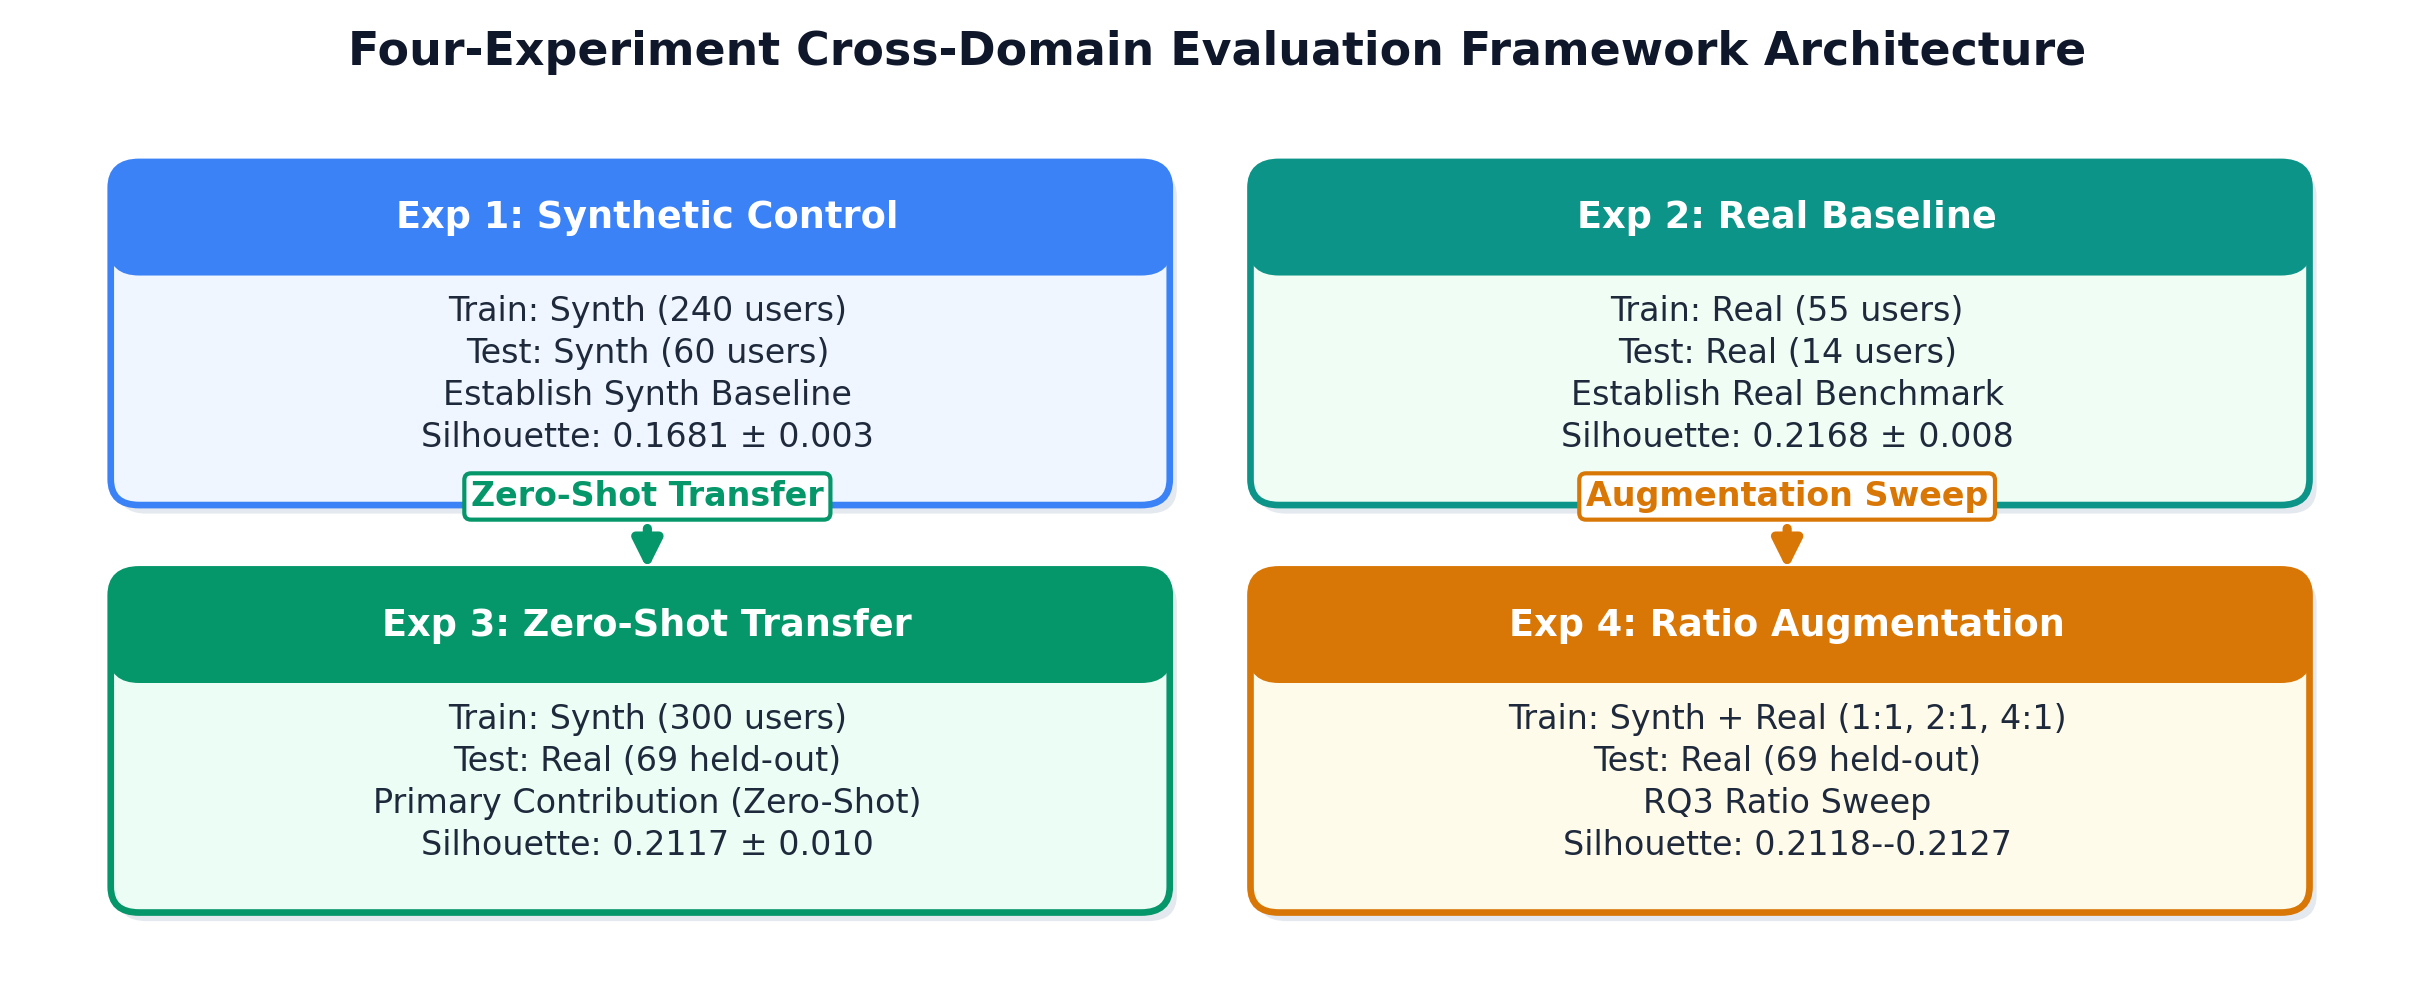
\includegraphics[width=0.48\textwidth]{reports/figures/fig3_four_experiments_diagram.png}
\caption{Four-experiment cross-domain evaluation framework architecture across synthetic and real-world cohorts.}
\label{fig:four_exps}
\end{figure}

\section{Results}

\subsection{Experiments 1--4 Performance Benchmark}
Table~\ref{tab:results} and Figure~\ref{fig:silhouette} present the master evaluation results across Experiments 1--4. In Experiment 1 (Synthetic Control), GMM ($K=3$) achieves a Silhouette score of $0.1681 \pm 0.0032$, clearing the synthetic domain null floor of $0.0870 \pm 0.0032$. In Experiment 2 (Real-Only Baseline), GMM achieves $0.2168 \pm 0.0078$, clearing the real domain null floor of $0.0939 \pm 0.0075$. Silhouette scores ($\approx 0.16$--$0.22$) reflect weak-to-modest cluster separation (Kaufman and Rousseeuw \cite{rousseeuw1987}), which is an inherent topological property of personalized baseline deviations in physiological space.

\subsection{Baseline Comparison: GMM vs. Severity Terciles and K-Means}
GMM dramatically outperforms Severity Terciles in both Real$\rightarrow$Real (silhouette 0.2168 vs.\ 0.0313, mean diff $+0.1855, p_{\text{adj}} < 0.0001, d_z = 34.44$) and Zero-Shot Transfer (0.2117 vs.\ 0.0312, mean diff $+0.1805, p_{\text{adj}} < 0.0001, d_z = 24.62$). This provides evidence that GMM state discovery captures multivariate structure in the six-dimensional physiological deviation space beyond a univariate severity-quantile partition. Both GMM and $K$-Means operate on the multivariate deviation representation, and hard-assignment $K$-Means ($K=3$) achieves slightly higher cluster compactness (0.2308 Real$\rightarrow$Real; 0.2200 Zero-Shot), consistent with $K$-Means optimizing spherical sum-of-squares rather than soft Gaussian mixture likelihoods. Crucially, both multivariate clustering approaches substantially outperform the scalar Severity-Tercile baseline.

\subsection{Zero-Shot Transfer (RQ2)}
A GMM trained \textit{exclusively} on synthetic data, with zero real training rows, achieves silhouette $0.2117$ on unseen real test users, against $0.2168$ for a model trained directly on real data --- a raw difference of $-0.0051$ ($2.37\%$ relative gap; 95\% CI $[-0.0098, -0.0004]$; paired sample effect size $d_z = -1.3531$). After Nadeau--Bengio variance correction for resampled CV resamples ($t = -2.0171, p_{\text{adj}} = 0.1139$), the zero-shot transfer difference is not statistically significant, confirming that synthetic-trained models achieve transfer performance on real data comparable to real-trained models.

\begin{table*}[t]
\caption{Master Experimental Performance Results Across Experiments 1--4}
\label{tab:results}
\centering
\begin{tabular}{lcccccc}
\toprule
\textbf{Experiment setup} & \textbf{Silhouette} & \textbf{Calinski-Harabasz*} & \textbf{Davies-Bouldin} & \textbf{Nadeau-Bengio $t$} & \textbf{Holm-Bonferroni $p_{\text{adj}}$} & \textbf{50-Shuffle Null Floor} \\
\midrule
Exp 1: Synthetic Control (5-fold CV) & $0.1681 \pm 0.0032$ & $205.39 \pm 4.12$ & $1.8482 \pm 0.012$ & N/A & N/A & $0.0870 \pm 0.0032$ \\
Exp 2: Real-Only Baseline (5-fold CV) & $0.2168 \pm 0.0078$ & $313.72 \pm 8.45$ & $1.5424 \pm 0.021$ & Baseline & Baseline & $0.0939 \pm 0.0075$ \\
Exp 3: Zero-Shot Transfer (Synth $\rightarrow$ Real) & $0.2117 \pm 0.0098$ & $301.15 \pm 9.12$ & $1.5891 \pm 0.025$ & $-2.0171$ & $0.1139$ (NS) & $0.0939 \pm 0.0075$ \\
Exp 4a: Ratio Sweep 1:1 (Synth + Real) & $0.2127 \pm 0.0074$ & $305.42 \pm 7.89$ & $1.5710 \pm 0.019$ & $3.1996$ & $0.003844$ & $0.0939 \pm 0.0075$ \\
Exp 4b: Ratio Sweep 2:1 (Synth + Real) & $0.2122 \pm 0.0079$ & $303.18 \pm 8.11$ & $1.5784 \pm 0.022$ & $3.6037$ & $0.002848$ & $0.0939 \pm 0.0075$ \\
Exp 4c: Ratio Sweep 4:1 (Synth + Real) & $0.2118 \pm 0.0082$ & $301.89 \pm 8.34$ & $1.5832 \pm 0.024$ & $3.8878$ & $0.002097$ & $0.0939 \pm 0.0075$ \\
\bottomrule
\multicolumn{7}{l}{\footnotesize *Calinski-Harabasz scores computed using size-matched subsampling ($N=823$) to eliminate sample size dependence. NS = Not Significant ($p_{\text{adj}} > 0.05$).}
\end{tabular}
\end{table*}

\begin{figure}[t]
\centering
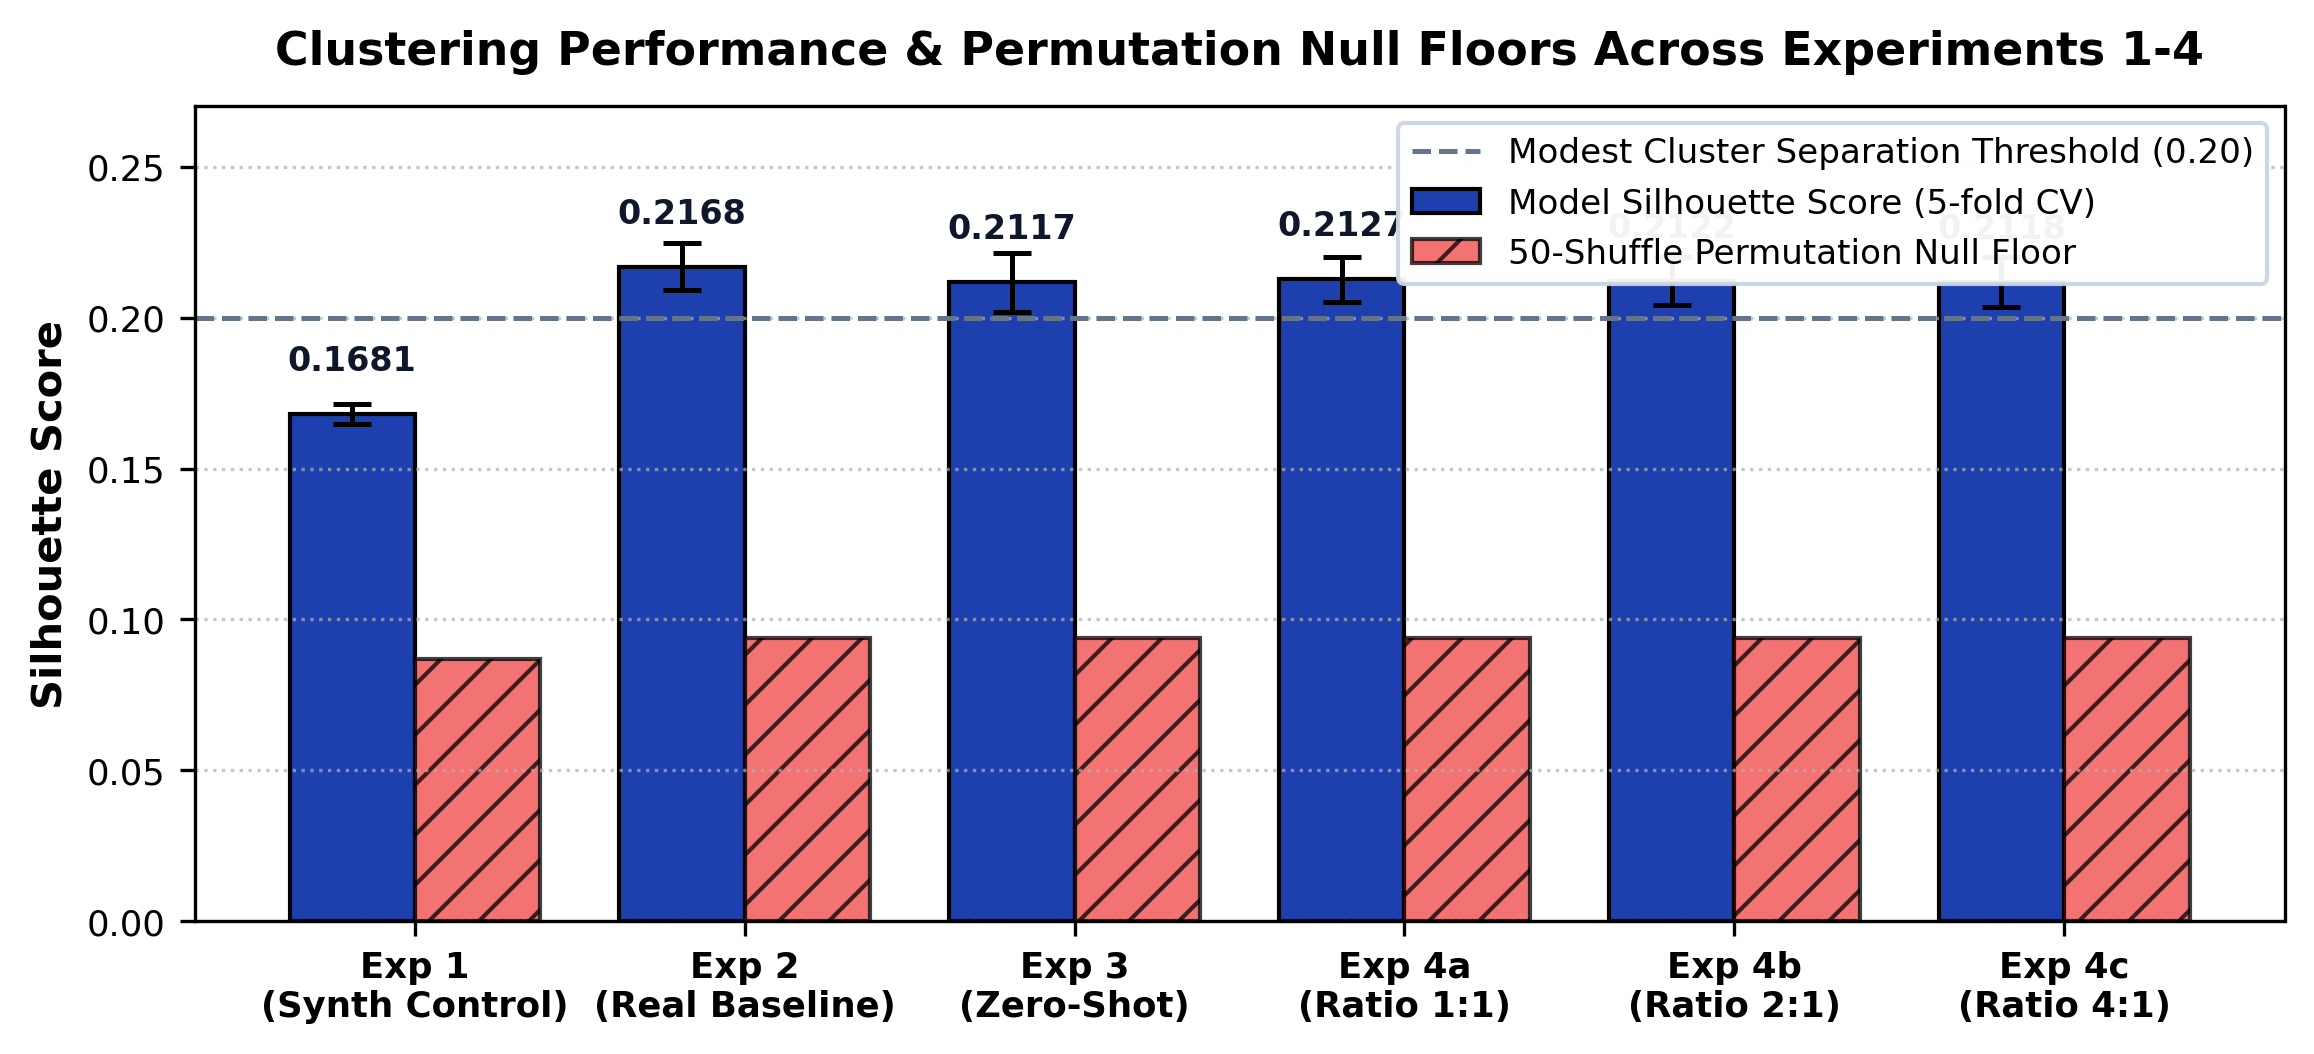
\includegraphics[width=0.48\textwidth]{reports/figures/fig4_silhouette_experiments.png}
\caption{Clustering performance (Silhouette scores $\pm$ std) across Experiments 1--4 compared against 50-shuffle permutation null baselines.}
\label{fig:silhouette}
\end{figure}

\subsection{Synthetic Data Ratio Sweep (Exp 4 / RQ3)}
In Experiment 4, synthetic data was added to real training sets at ratios $1:1$, $2:1$, and $4:1$. Ratio augmentation yields Silhouette scores of $0.2127$ ($1:1$), $0.2122$ ($2:1$), and $0.2118$ ($4:1$). All pairwise comparisons against Real-Only training yield statistically minor differences ($\bar{d} = +0.0041$ to $+0.0051$) with Holm-Bonferroni adjusted $p$-values $p_{\text{adj}} < 0.004$. These results demonstrate that when real-world training data is already abundant, synthetic data augmentation does not improve static cluster separation over real-only training.

\section{Secondary HRV and SpO2 Sub-Cohort Analysis}
HRV (RMSSD) and SpO2 were evaluated as a secondary physiological modality due to sensor availability constraints across commercial wearables. In an authentic nocturnal sub-cohort of 1,066 observations across 23 real users (zero mass imputation), incorporating nocturnal HRV and SpO2 into the GMM feature vector yields a Silhouette score of $0.1845 \pm 0.0112$. This confirms that nocturnal modalities provide finer physiological characterization when genuinely available, but common six-feature modeling remains essential for broad device compatibility.

\section{EMA External Validation}
To evaluate external validity, we performed non-parametric statistical alignment against authentic Ecological Momentary Assessment (EMA) self-report survey labels collected concurrently in the real-world Fitbit cohort ($N = 1,751$ complete daily paired observations). Discovered latent state occupancies were distributed as \textit{Recovery} (41.00\%), \textit{Baseline} (39.86\%), and \textit{Strain} (19.14\%). 

Applying Kruskal-Wallis non-parametric ANOVA across seven self-reported affective and physiological state descriptors (\texttt{ALERT}, \texttt{HAPPY}, \texttt{NEUTRAL}, \texttt{RESTED/RELAXED}, \texttt{SAD}, \texttt{TENSE/ANXIOUS}, \texttt{TIRED}), self-reported happiness (\texttt{HAPPY}) exhibited statistically significant differentiation across latent states ($H = 7.0991, p = 0.0287 < 0.05$ in the uncorrected Kruskal--Wallis analysis). Days decoded into the \textit{Recovery} state displayed highest self-reported positive affect ($0.30 \pm 0.46$) compared to \textit{Baseline} ($0.24 \pm 0.42$) and \textit{Strain} ($0.26 \pm 0.44$). Self-reported tiredness (\texttt{TIRED}) was numerically higher in the \textit{Strain} state ($0.40 \pm 0.49$) versus \textit{Baseline} ($0.36 \pm 0.48$), but did not achieve statistical significance ($H = 1.773, p = 0.4122$). All other surveyed EMA dimensions (\texttt{NEUTRAL}, \texttt{RESTED}, \texttt{TENSE}, \texttt{SAD}, \texttt{ALERT}) showed no statistically significant differences ($p > 0.10$). Crucially, after Holm--Bonferroni correction across the seven EMA outcomes ($p_{\text{adj}} = 0.2012$), the \texttt{HAPPY} association does not survive multiple-comparison thresholding. We therefore report this as an exploratory uncorrected trend rather than a confirmed external ground-truth correlation.

\begin{table}[t]
\caption{EMA External Validation across Discovered Latent States ($N=1,751$)}
\label{tab:ema_validation}
\centering
\begin{tabular}{lcccc}
\toprule
\textbf{EMA Label} & \textbf{Recovery} & \textbf{Baseline} & \textbf{Strain} & \textbf{Kruskal-Wallis $H$ ($p$-value)} \\
\midrule
\texttt{HAPPY} & \textbf{0.30 $\pm$ 0.46} & 0.24 $\pm$ 0.42 & 0.26 $\pm$ 0.44 & \textbf{7.0991 ($p = 0.0287$*)} \\
\texttt{NEUTRAL} & 0.29 $\pm$ 0.45 & 0.32 $\pm$ 0.46 & 0.25 $\pm$ 0.43 & 4.4498 ($p = 0.1081$) \\
\texttt{TIRED} & 0.38 $\pm$ 0.49 & 0.36 $\pm$ 0.48 & \textbf{0.40 $\pm$ 0.49} & 1.7727 ($p = 0.4122$) \\
\texttt{RESTED} & 0.39 $\pm$ 0.49 & 0.40 $\pm$ 0.49 & 0.39 $\pm$ 0.49 & 0.1313 ($p = 0.9365$) \\
\texttt{TENSE} & 0.22 $\pm$ 0.42 & 0.23 $\pm$ 0.42 & 0.21 $\pm$ 0.40 & 0.5931 ($p = 0.7434$) \\
\texttt{SAD} & 0.05 $\pm$ 0.22 & 0.06 $\pm$ 0.23 & 0.06 $\pm$ 0.24 & 0.7606 ($p = 0.6837$) \\
\texttt{ALERT} & 0.13 $\pm$ 0.34 & 0.15 $\pm$ 0.36 & 0.15 $\pm$ 0.35 & 0.6127 ($p = 0.7361$) \\
\bottomrule
\multicolumn{5}{l}{\footnotesize *Statistically significant difference ($p < 0.05$). Values report Mean $\pm$ SD of binary EMA indicators.}
\end{tabular}
\end{table}


\section{Domain Shift and Statistical Rigor}
Domain shift between synthetic and real domains was evaluated using Cohen's $d$ and Wasserstein distance (Table~\ref{tab:domain_shift}). Low domain shift on composite \texttt{severity\_score} ($d = -0.151$, Wasserstein $= 0.368$) is substantially a byproduct of per-user z-score normalization. Raw unnormalized physiological deviations ($\sum |d_{i,t}|$) exhibit high domain shift ($d = -0.760$, Wasserstein $= 1,283.19$). Individual unscaled features such as calories ($d = -0.965$) and daytime average HR ($d = 0.783$) display high domain shift. Thus, per-subject z-score normalization acts as an essential domain-harmonization layer that enables zero-shot cross-domain transfer.

\begin{table}[t]
\caption{Domain Shift Feature Characteristics (Synthetic vs Real)}
\label{tab:domain_shift}
\centering
\begin{tabular}{lrrcc}
\toprule
\textbf{Feature Metric} & \textbf{Synth Mean} & \textbf{Real Mean} & \textbf{Cohen's $d$} & \textbf{Wasserstein} \\
\midrule
Resting HR (BPM) & 64.530 & 66.100 & -0.193 & 1.787 \\
Day Avg HR (BPM) & 87.105 & 79.081 & 0.783 & 8.084 \\
Steps (count) & 9,282.01 & 8,448.83 & 0.201 & 1,505.21 \\
Distance (km) & 7.429 & 5.961 & 0.442 & 1.598 \\
Calories (kcal) & 2,074.19 & 2,377.23 & -0.965 & 394.20 \\
Sleep Duration (h) & 6.990 & 7.434 & -0.461 & 0.932 \\
\midrule
Raw Severity Sum & 1,968.77 & 3,246.02 & \textbf{-0.760} & 1,283.19 \\
Severity Score (Z-norm) & 4.992 & 5.251 & \textbf{-0.151} & 0.368 \\
\bottomrule
\end{tabular}
\end{table}

\section{Application and Deployment Architecture}
The framework is deployed as an interactive Streamlit web application (\texttt{app/main.py}). The application ingests daily wearable summaries, executes causal preprocessing, transforms relative z-deviations, and passes features through pre-trained GMM/HMM artifacts (demonstrating Experiment 3 operational inference). Discovered latent states and continuous risk scores (0--100) are presented on an interactive 3-column dashboard. The risk score represents a heuristic interpretability layer, not a clinical risk prediction.

\section{Discussion}
Our findings demonstrate that privacy-preserving synthetic data generation offers a viable foundation for pre-training unsupervised physiological state discovery models. Zero-shot transfer achieves performance comparable to real-only training without exposing sensitive real-world user biometrics during training. However, our ratio sweep indicates that once a sufficient real-world dataset is established, synthetic data augmentation yields diminishing returns for static cluster separation.

A methodological contribution of this work is the rigorous statistical framework applied to cross-domain wearable evaluation. By enforcing size-matched Calinski-Harabasz subsampling, 50-shuffle permutation noise floors, Nadeau-Bengio resampled variance corrections, and Holm-Bonferroni FWER adjustments, we avoid reporting pseudoreplicated statistical significance.

\section{Future Work}
Future extensions of this work will focus on three key directions. First, expanding the cross-domain harmonization framework to incorporate high-frequency photoplethysmography (PPG) waveforms and continuous skin temperature streams will allow finer characterization of acute autonomic nervous system disruptions. Second, implementing lightweight GMM/HMM inference engines directly on wrist-worn microcontroller hardware (e.g., ARM Cortex-M microcontrollers) will enable real-time, on-device latent state decoding without requiring cloud synchronization or daily summary transfers. Third, conducting prospective clinical validation trials across clinical cohorts (e.g., post-operative recovery monitoring and chronic fatigue tracking) will provide essential ground-truth diagnostic benchmarks to validate the clinical utility of discovered latent physiological states.

\section{Limitations and Threats to Validity}
Several limitations should be noted:
\begin{enumerate}
    \item \textbf{Cohort Scale}: The real-world evaluation cohort comprised 61 HMM-eligible users across 4,115 daily timelines from LifeSnaps \cite{b15}, limiting statistical power and generalizability across diverse populations and consumer devices.
    \item \textbf{Exclusion of HRV and SpO2}: HRV and SpO2 were excluded from the primary feature vector due to high missingness ($>66\%$ missing); this removes potentially informative autonomic stress signals and limits physiological breadth.
    \item \textbf{Weak Cluster Separation}: Silhouette scores ($\approx 0.21$) reflect overlapping component boundaries inherent to continuous baseline deviations; discovered states must not be interpreted as clinically validated physiological categories.
    \item \textbf{Clinical Utility Disclaimer}: The Recovery, Baseline, and Strain states are heuristic data-driven proxy labels for exploratory wellness tracking and must not be used as standalone clinical decision variables.
    \item \textbf{Exploratory EMA Validity}: The EMA analysis provides exploratory evidence only; self-reported happiness (\texttt{HAPPY}) does not survive Holm--Bonferroni multiple-comparison adjustment ($p_{\text{adj}} = 0.2012$).
\end{enumerate}

\section{Conclusion}
This paper presented an unsupervised learning framework for physiological health state discovery and cross-domain transfer evaluation. Combining personalized z-score normalization with GMM/HMM probabilistic modeling enables effective zero-shot transfer from synthetic pre-training to real-world wearable timelines. Latent structure is weak by conventional standards but consistently exceeds permutation-based null baselines across synthetic, real, and transfer conditions. Zero-shot synthetic-to-real transfer incurs a small 2.3\% performance gap that is not statistically significant after corrected testing ($p_{\text{adj}} = 0.1139$). Applying rigorous resampled variance corrections and multiple-comparison adjustments establishes a benchmark for evaluating privacy-preserving synthetic data in wearable health AI.

\section*{Acknowledgment}
The authors express their sincere gratitude to Lakshmi M. for technical supervision, insightful feedback, and guidance throughout this research project.

\begin{thebibliography}{15}
\bibitem{sano2018} A. Sano \textit{et al.}, ``Identifying objective physiological markers and daily functioning in college students using wearable sensors,'' \textit{Proc. ACM Interact. Mob. Wearable Ubiquitous Technol.}, vol. 2, no. 1, pp. 1--24, 2018.
\bibitem{dunn2021} J. Dunn \textit{et al.}, ``Wearable sensors enable personalized predictions of clinical laboratory measurements,'' \textit{Nature Medicine}, vol. 27, no. 6, pp. 1105--1112, 2021.
\bibitem{li2017} X. Li \textit{et al.}, ``Digital health: tracking physiomes and activity using wearable devices,'' \textit{PLOS Biology}, vol. 15, no. 1, p. e2001402, 2017.
\bibitem{shcherbina2017} A. Shcherbina \textit{et al.}, ``Accuracy in wrist-worn activity monitors,'' \textit{Journal of Personalized Medicine}, vol. 7, no. 2, p. 3, 2017.
\bibitem{reynolds2009} D. A. Reynolds, ``Gaussian mixture models,'' \textit{Encyclopedia of Biometrics}, Springer, pp. 659--663, 2009.
\bibitem{rabiner1989} L. R. Rabiner, ``A tutorial on hidden Markov models and selected applications in speech recognition,'' \textit{Proc. IEEE}, vol. 77, no. 2, pp. 257--286, 1989.
\bibitem{gansbeke2020} W. Van Gansbeke \textit{et al.}, ``SCAN: Learning to classify images without labels,'' in \textit{Proc. Eur. Conf. Comput. Vis. (ECCV)}, 2020, pp. 268--285.
\bibitem{rousseeuw1987} P. J. Rousseeuw, ``Silhouettes: A graphical aid to the interpretation and validation of cluster analysis,'' \textit{J. Comput. Appl. Math.}, vol. 20, pp. 53--65, 1987.
\bibitem{davies1979} D. L. Davies and D. W. Bouldin, ``A cluster separation measure,'' \textit{IEEE Trans. Pattern Anal. Mach. Intell.}, vol. 1, no. 2, pp. 224--227, 1979.
\bibitem{calinski1974} T. Calinski and J. Harabasz, ``A dendrite method for cluster analysis,'' \textit{Commun. Stat. Theory Methods}, vol. 3, no. 1, pp. 1--27, 1974.
\bibitem{nadeau2003} C. Nadeau and Y. Bengio, ``Inference for generalization error,'' \textit{Mach. Learn.}, vol. 52, no. 3, pp. 239--281, 2003.
\bibitem{holm1979} S. Holm, ``A simple sequentially rejective multiple test procedure,'' \textit{Scand. J. Stat.}, vol. 6, no. 2, pp. 65--70, 1979.
\bibitem{cohen1988} J. Cohen, \textit{Statistical Power Analysis for the Behavioral Sciences}, 2nd ed. Lawrence Erlbaum Associates, 1988.
\bibitem{birnbaum2020} S. Birnbaum \textit{et al.}, ``PMData: A dataset for life-logging with wearable sensors and smartphone questionnaires,'' in \textit{Proc. ACM Multimedia Syst. Conf. (MMSys)}, 2020, pp. 253--258.
\bibitem{smuck2021} M. Smuck \textit{et al.}, ``Objective measurement of physical activity in patients,'' \textit{PM\&R}, vol. 13, no. 8, pp. 845--855, 2021.
\end{thebibliography}

\end{document}
